\section{Radds存储系统详细设计与实现}

	本章对存储系统的各层进行详细设计与实现,针对各层内部的子系统,各层之间的接口进行详细定义。

	\subsection{基础层详细设计与实现}
	
   		\subsubsection{错误处理的实现}

		针对go语言本身的特性,错误处理成为整个系统程序开发的首要项目,我们以轻量化,插件化的形式进行错误处理。
	
		\begin{lstlisting}[caption=Errors , label=code_radds_errors]

 
		\end{lstlisting}                 

	
			
   		\subsubsection{日志系统的实现}
    
	   	为了防止写入内存的数据库因为进程异常、操作系统掉电等情况发生丢失,
	   	存储系统在写内存之前会将本次写操作的内容写入日志文件中。
    
    	\begin{figure}[H]
    		\centering
    		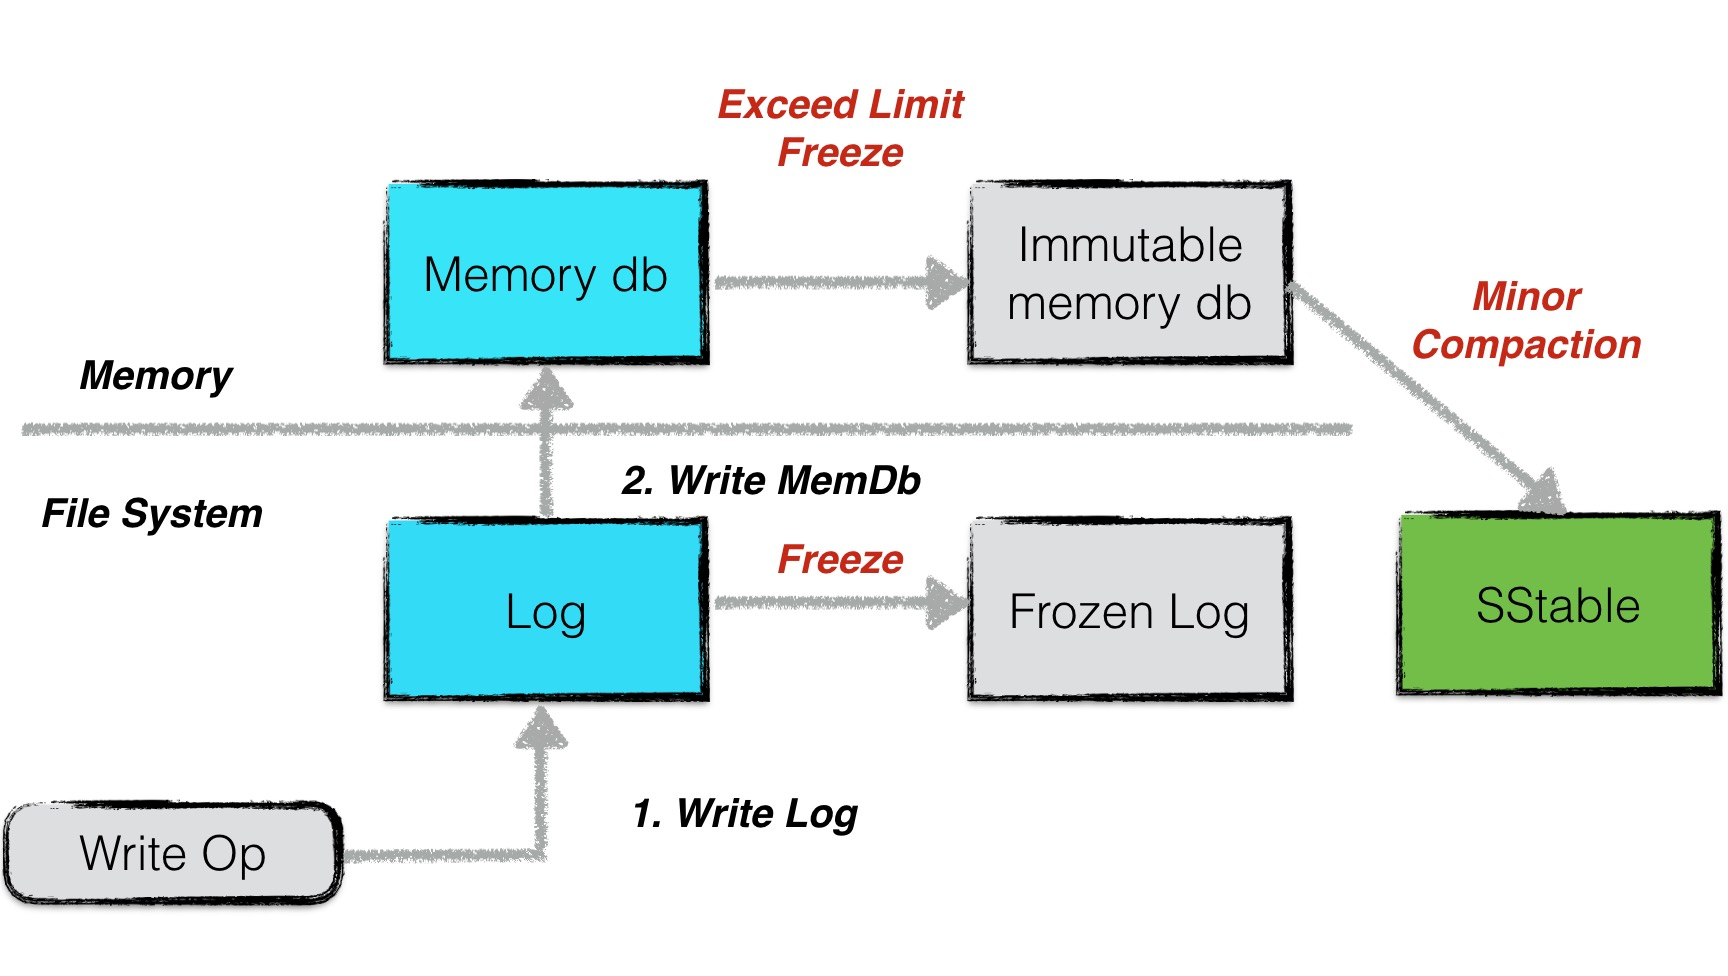
\includegraphics[width=0.95\textwidth]{images/two_log}
    		\caption{日志系统架构图}
    		\label{two_log}
    	\end{figure}
		存储系统中,有两个memory db,以及对应的两份日志文件。
		其中一个memory db是可读写的,当这个db的数据量超过预定的上限时,
		便会转换成一个不可写的memory db,与此同时,与之对应的日志文件也变成一份frozen log。

		而新生成的immutable memory db则会由后台的minor compaction进程将其转换成一个sstable文件进行持久化,
		持久化完成,与之对应的frozen log被删除。
    
		\begin{enumerate}
		\item 日志结构

		\begin{figure}[H]
			\centering
			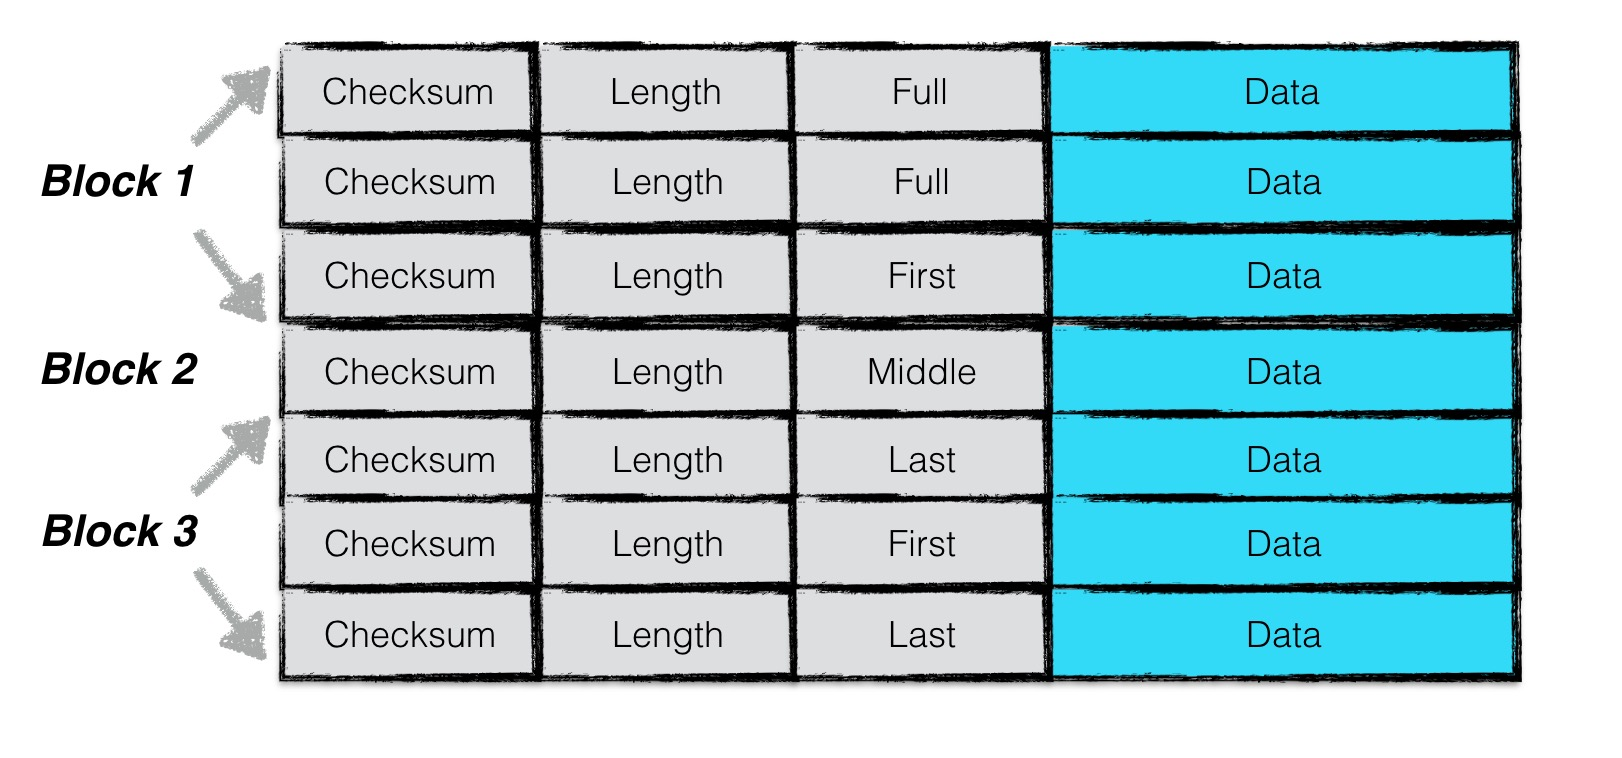
\includegraphics[width=0.95\textwidth]{images/journal}
			\caption{日志文件存储结构图}
			\label{journal}
		\end{figure}
		为了增加读取效率,日志文件中按照block进行划分,每个block的大小为32KiB。
		每个block中包含了若干个完整的chunk。
		
		一条日志记录包含一个或多个chunk。
		每个chunk包含了一个7字节大小的header,前4字节是该chunk的校验码,
		紧接的2字节是该chunk数据的长度,以及最后一个字节是该chunk的类型。
		其中checksum校验的范围包括chunk的类型以及随后的data数据。
	
		chunk共有四种类型:full,first,middle,last。
		一条日志记录若只包含一个chunk,则该chunk的类型为full。
		若一条日志记录包含多个chunk,则这些chunk的第一个类型为first, 
		最后一个类型为last,中间包含大于等于0个middle类型的chunk。
		
		由于一个block的大小为32KiB,因此当一条日志文件过大时,
		会将第一部分数据写在第一个block中,且类型为first,
		若剩余的数据仍然超过一个block的大小,则第二部分数据写在第二个block中,
		类型为middle,最后剩余的数据写在最后一个block中,类型为last。
		
		\item 日志内容
		
		日志的内容为写入的batch编码后的信息。

		具体的格式为:

		\begin{figure}[H]
			\centering
			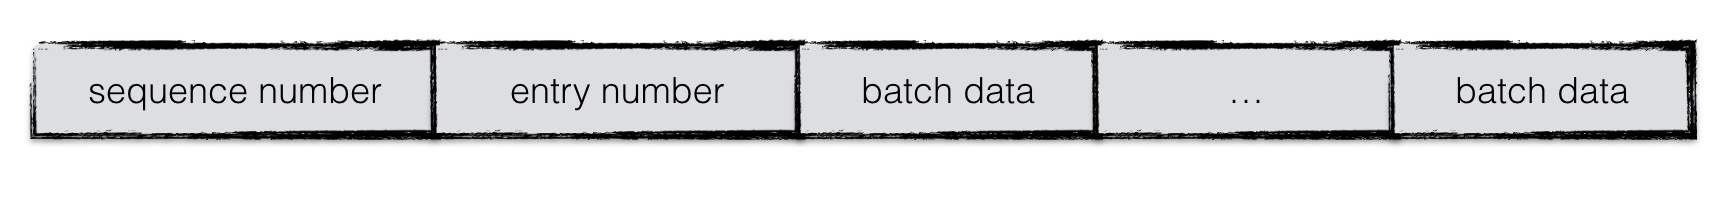
\includegraphics[width=0.95\textwidth]{images/journal_content}
			\caption{日志文件格式图}
			\label{journal_content}
		\end{figure}

		一条日志记录的内容包含:Header和Data
		其中Header中有(1)当前db的sequence number(2)本次日志记录中所包含的put/del操作的个数。
		
		紧接着写入所有batch编码后的内容。
		\item 日志文件写 
		
		\begin{figure}[H]
			\centering
			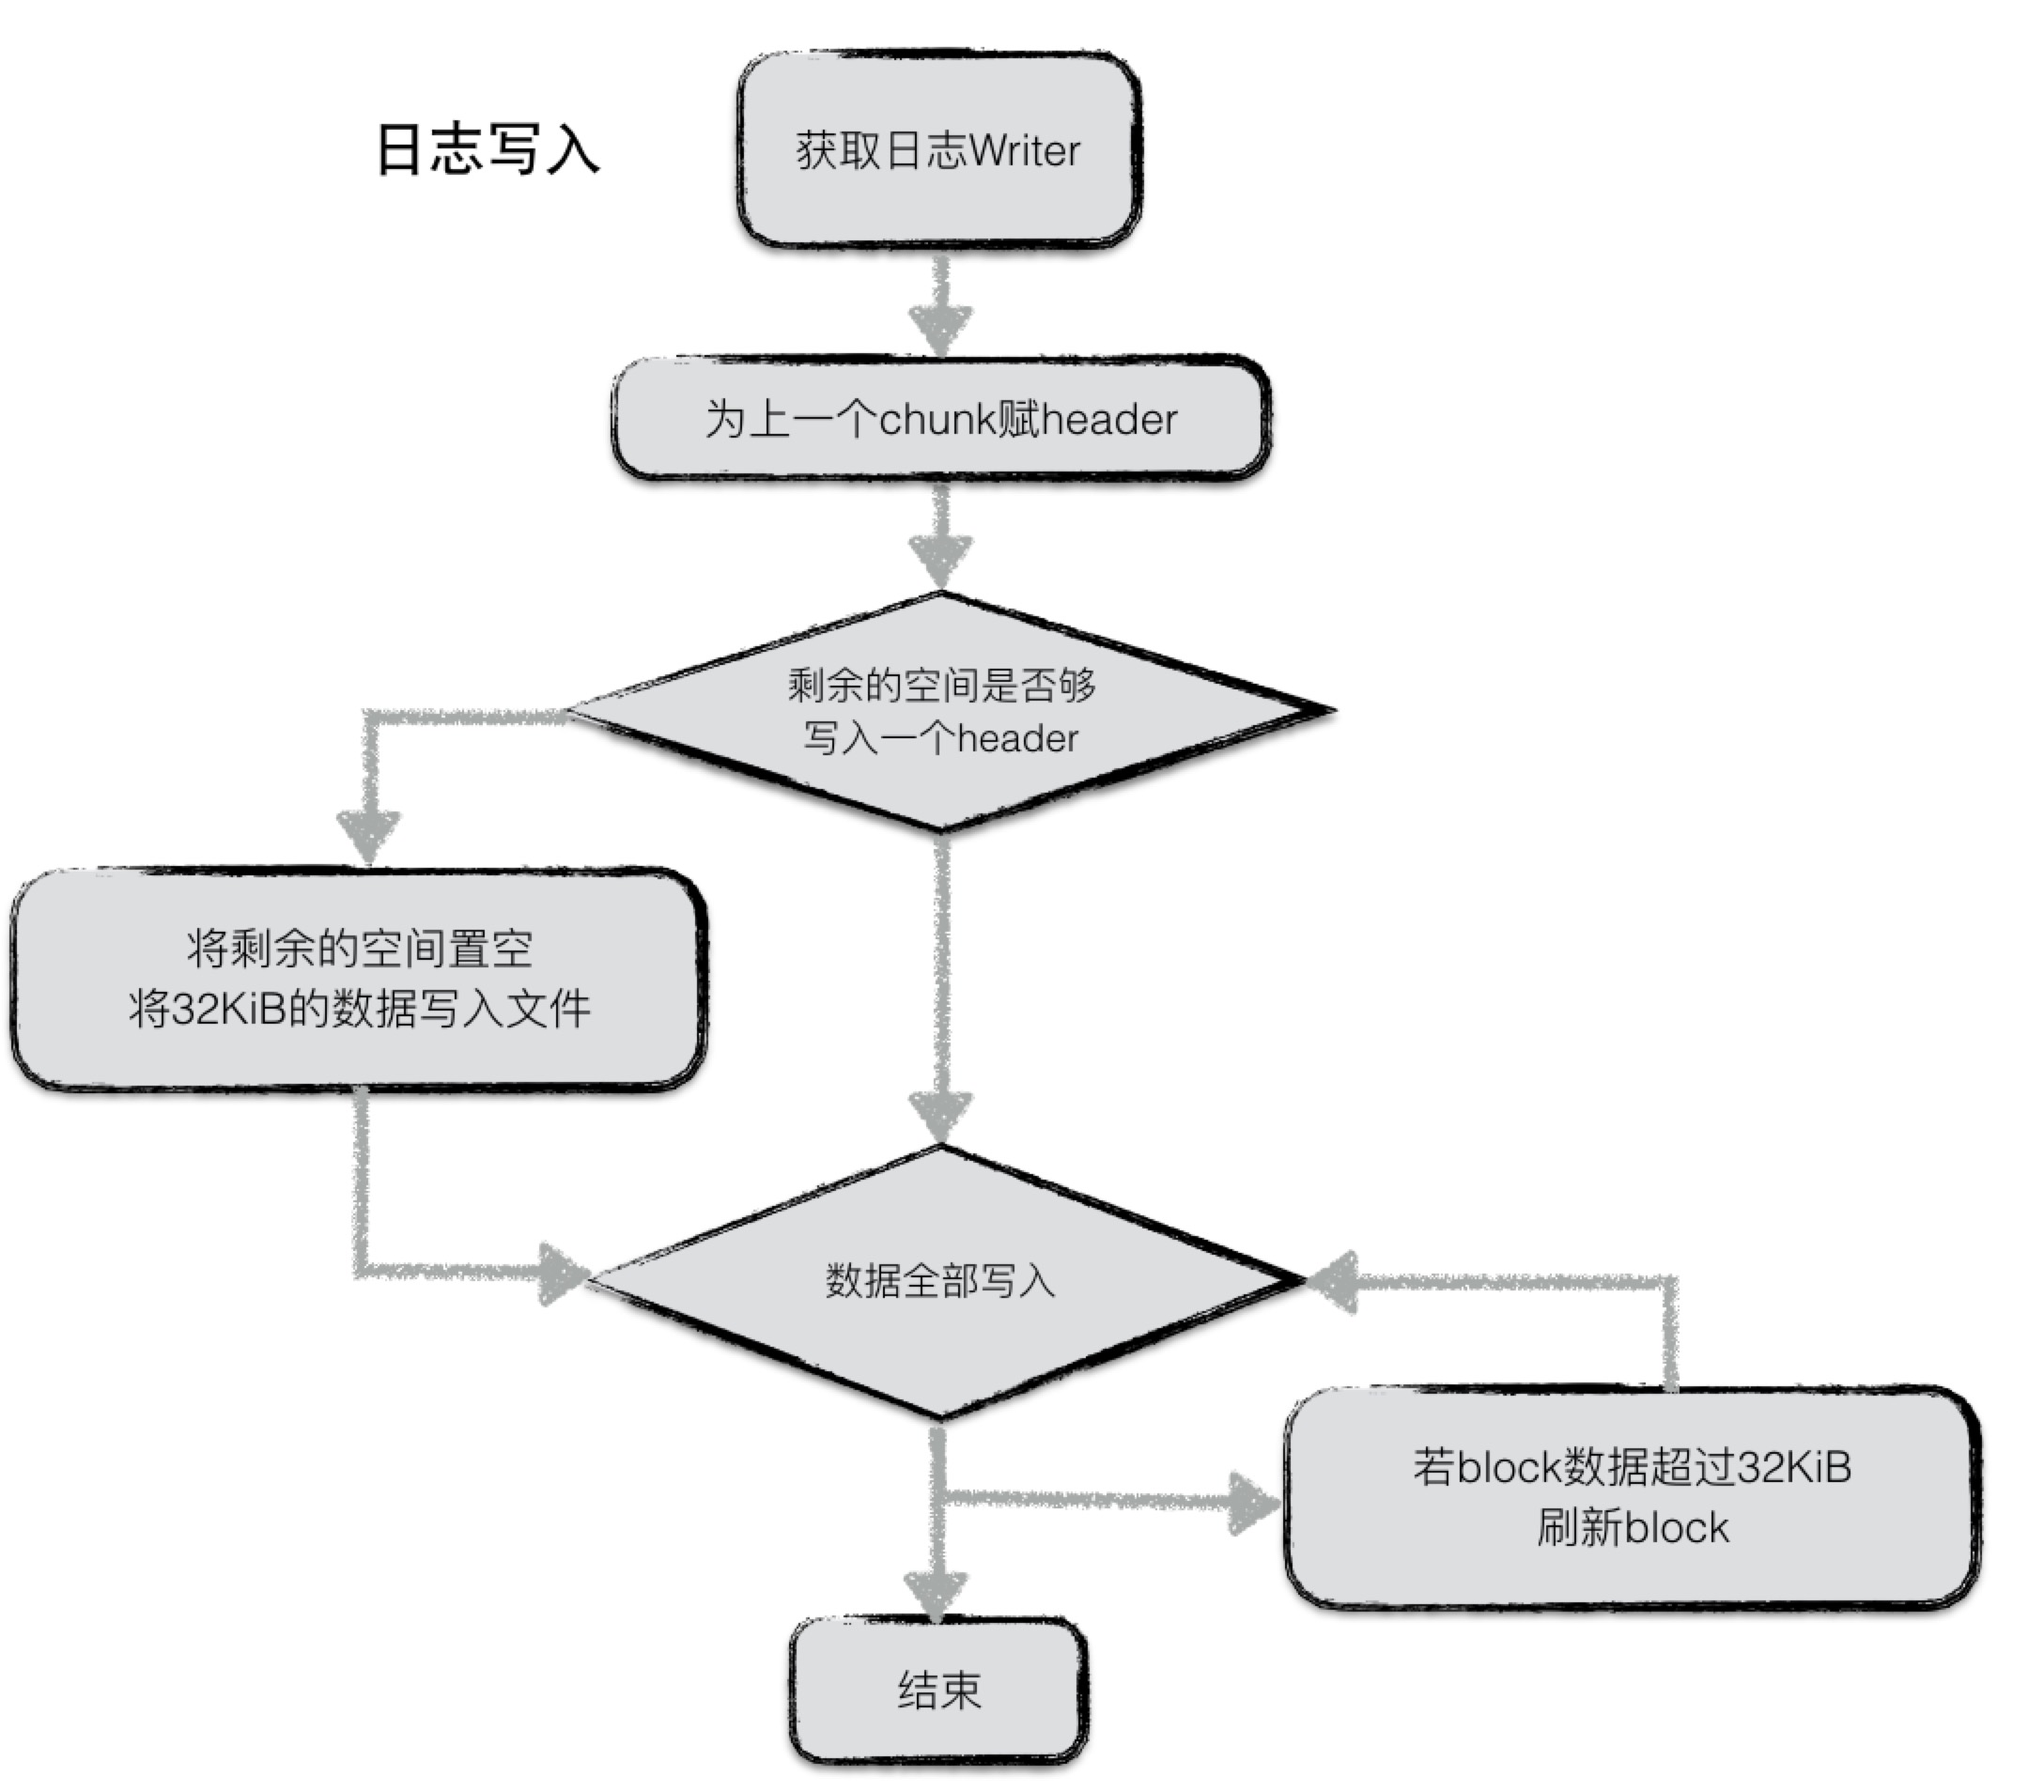
\includegraphics[width=0.95\textwidth]{images/journal_write}
			\caption{日志文件写流程图}
			\label{journal_write}
		\end{figure}
		
		日志写入流程较为简单,在存储系统内部,实现了一个journal的writer。
		首先调用Next函数获取一个singleWriter,
		这个singleWriter的作用就是写入一条journal记录。

		singleWriter开始写入时,标志着第一个chunk开始写入。
		在写入的过程中,不断判断writer中buffer的大小,若超过32KiB,
		将chunk开始到现在做为一个完整的chunk,为其计算header之后将整个chunk写入文件。
		与此同时reset buffer,开始新的chunk的写入。

		若一条journal记录较大,则可能会分成几个chunk存储在若干个block中。

		\item 日志文件读 
		
		同样,日志读取也较为简单。为了避免频繁的IO读取,每次从文件中读取数据时,
		按block(32KiB)进行块读取。

		每次读取一条日志记录,reader调用Next函数返回一个singleReader。
		singleReader每次调用Read函数就返回一个chunk的数据。每次读取一个chunk,
		都会检查这批数据的校验码、数据类型、数据长度等信息是否正确,若不正确,
		且用户要求严格的正确性,则返回错误,否则丢弃整个chunk的数据。

		循环调用singleReader的read函数,直至读取到一个类型为Last的chunk,
		表示整条日志记录都读取完毕,返回。

		\begin{figure}[H]
			\centering
			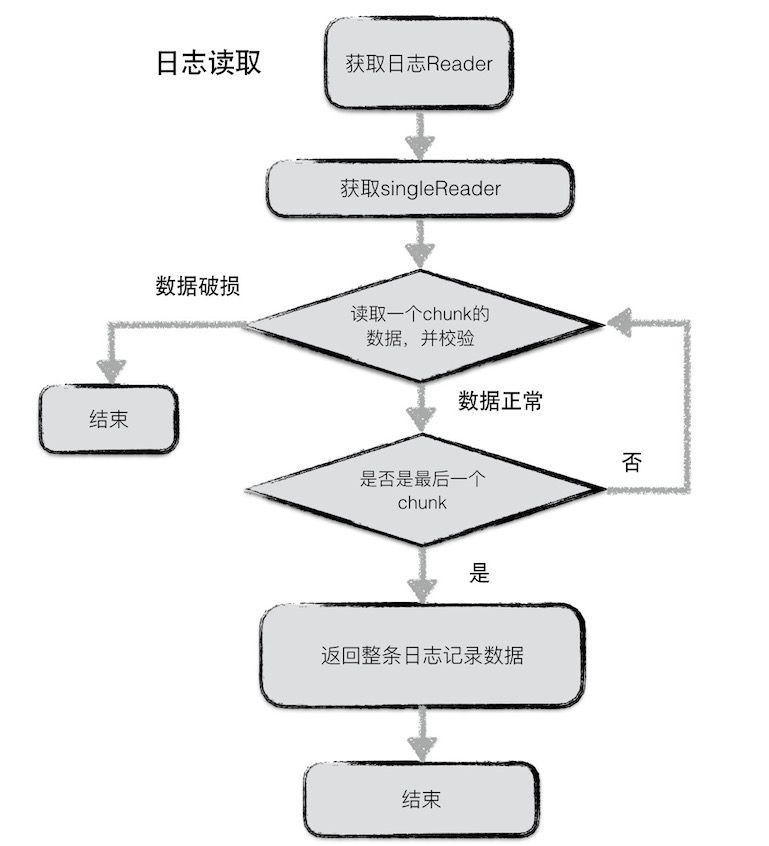
\includegraphics[width=0.95\textwidth]{images/journal_read}
			\caption{日志文件读流程图}
			\label{journal_read}
		\end{figure}
		
		
	
		\end{enumerate}
	
   		\subsubsection{其他工具库的实现}
    


  	\subsection{存储层详细设计与实现}
	
		\subsubsection{写数据的实现}
		
		\begin{enumerate}
		\item 写入数据的整体流程
			
		先来分析一下存储系统整个写入的流程,底层数据结构的支持以及为何能够优化我们的写入性能。
		
		\begin{figure}[H]
			\centering
			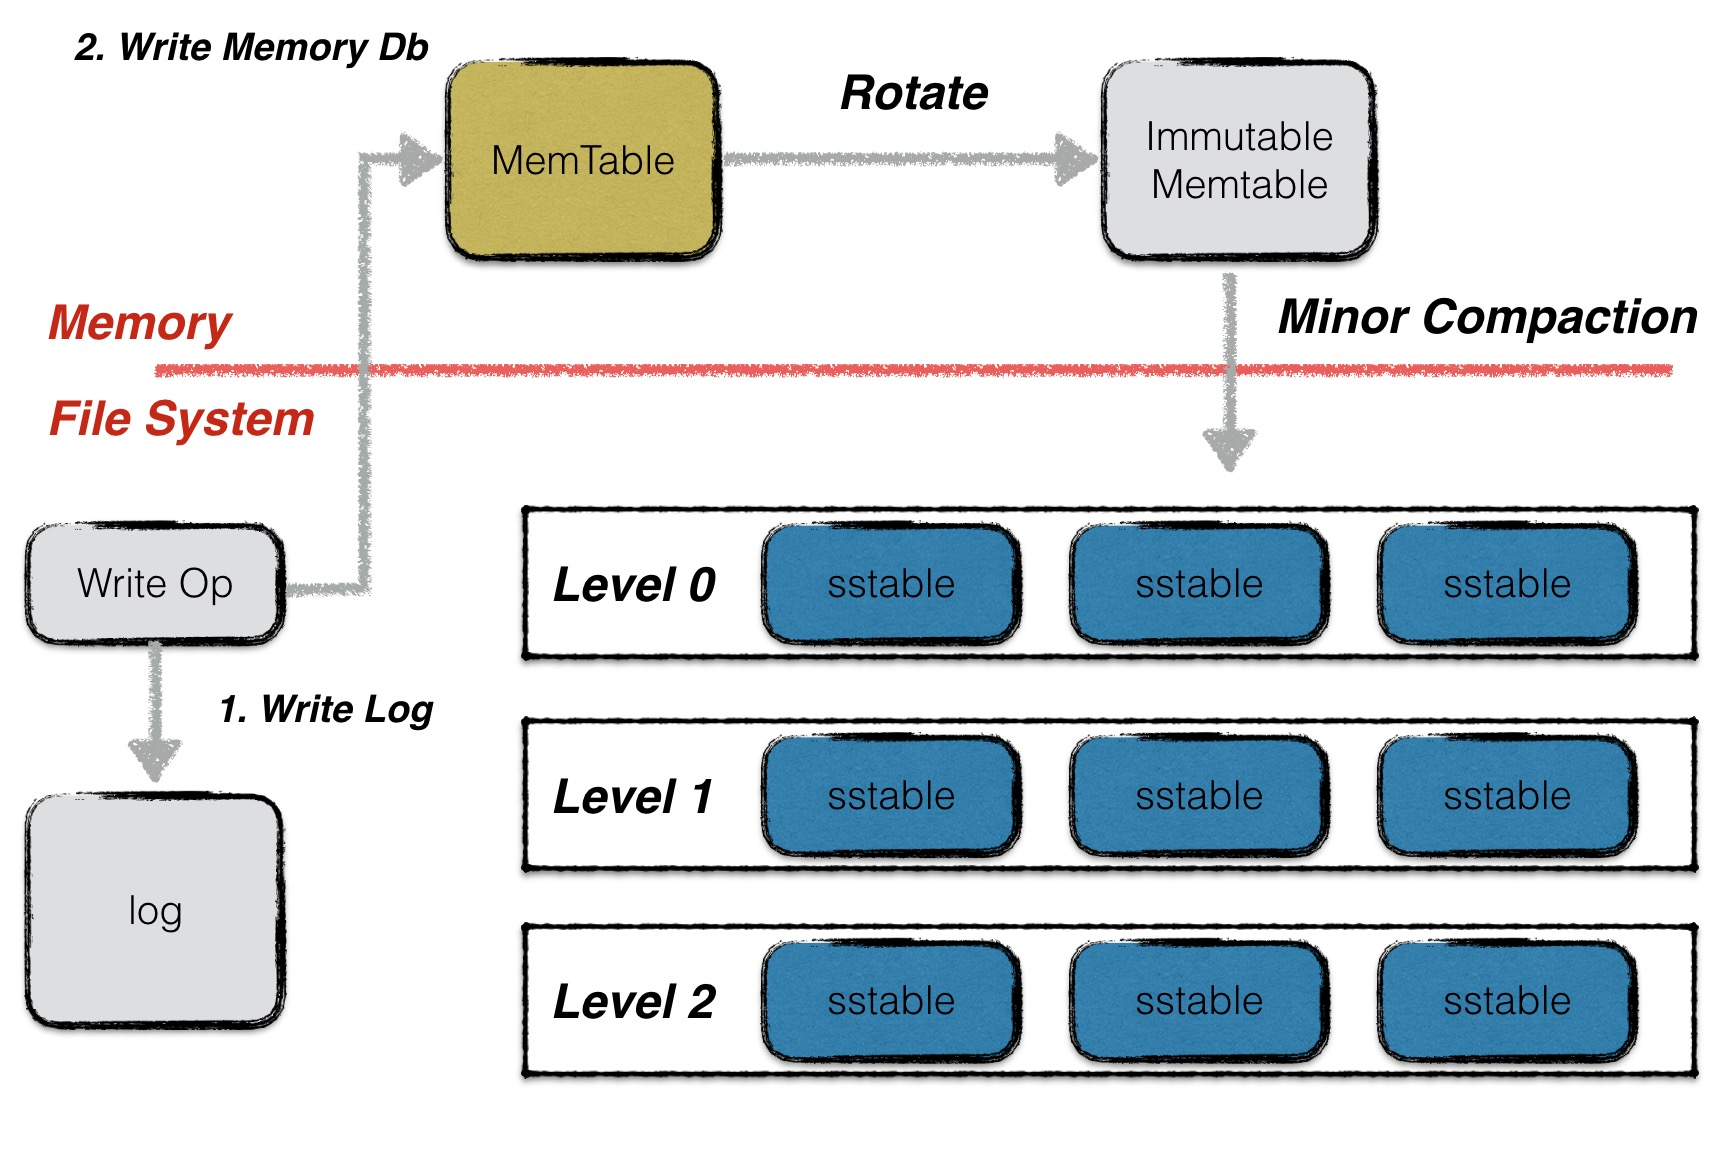
\includegraphics[width=0.95\textwidth]{images/write_op}
			\caption{存储系统写数据流程}
			\label{write_op}
		\end{figure}

		数据的一次写入分为两部分:

		将写操作写入日志;
		将写操作应用到内存数据库中;
		之前已经阐述过为何这样的操作可以优化写入性能,以及通过先写日志的方法能够保障用户的写入不丢失。

		其实仍然存在写入丢失的隐患。在写设置为非同步的情况下,在写完日志文件以后,
		操作系统并不是直接将这些数据真正落到磁盘中,而是暂时留在操作系统缓存中,
		因此当用户写入操作完成,操作系统还未来得及落盘的情况下,发生系统宕机,就会造成写丢失;
		但是若只是进程异常退出,则不存在该问题。

		\item 写类型
		
		由于是键值型非关系型数据存储,存储系统对外提供的写入接口有:
		(1)Put(2)Delete两种。这两种本质对应同一种操作,
		Delete操作同样会被转换成一个value为空的Put操作。
	
		除此以外,我们还提供了一个批量处理的工具Batch,用户可以依据Batch来完成批量更新操作,
		且这些操作是原子性的。

		\item batch结构
		
		无论是Put/Del操作,还是批量操作,
		底层都会为这些操作创建一个batch实例作为一个数据库操作的最小执行单元。
		因此首先介绍一下batch的组织结构。

		\begin{figure}[H]
			\centering
			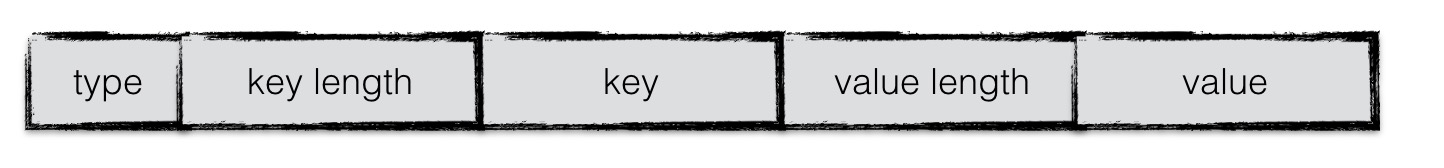
\includegraphics[width=0.95\textwidth]{images/batch}
			\caption{batch的数据结构}
			\label{batch}
		\end{figure}

		在batch中,每一条数据项都按照上图格式进行编码。
		每条数据项编码后的第一位是这条数据项的类型(更新还是删除),
		之后是数据项key的长度,数据项key的内容;若该数据项不是删除操作,
		则再加上value的长度,value的内容。

		batch中会维护一个size值,用于表示其中包含的数据量的大小。
		该size值为所有数据项key与value长度的累加,以及每条数据项额外的8个字节。
		这8个字节用于存储一条数据项额外的一些信息。
		

		\item key值编码
		
		当数据项从batch中写入到内存数据库中时,需要将一个key值的转换,即在存储系统内部,
		所有数据项的key是经过特殊编码的,这种格式称为internalKey。

		\begin{figure}[H]
			\centering
			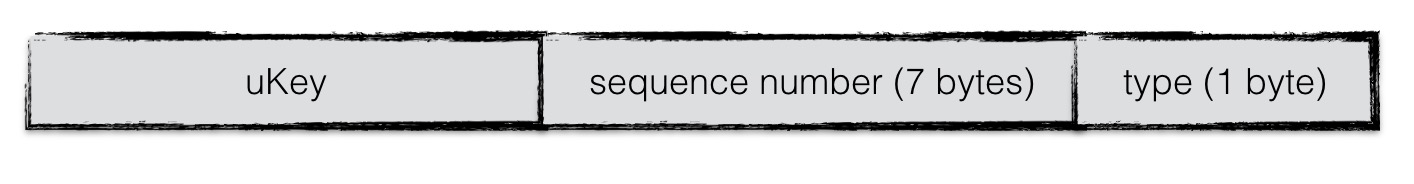
\includegraphics[width=0.95\textwidth]{images/internalkey}
			\caption{internalkey的数据结构}
			\label{internalkey}
		\end{figure}


		internalkey在用户key的基础上,尾部追加了8个字节,
		用于存储(1)该操作对应的sequence number(2)该操作的类型。

		其中,每一个操作都会被赋予一个sequence number。
		该计时器是在存储系统内部维护,每进行一次操作就做一个累加。
		由于在存储系统中,一次更新或者一次删除,采用的是append的方式,
		并非直接更新原数据。因此对应同样一个key,会有多个版本的数据记录,
		而最大的sequence number对应的数据记录就是最新的。

		此外,存储系统的快照(snapshot)也是基于这个sequence number实现的,
		即每一个sequence number代表着数据库的一个版本。

		\item 数据合并写入
		
		存储系统中,在面对并发写入时,做了一个处理的优化。
		在同一个时刻,只允许一个写入操作将内容写入到日志文件以及内存数据库中。
		为了在写入进程较多的情况下,减少日志文件的小写入,增加整体的写入性能,
		存储系统将一些“小写入”合并成一个“大写入”。

		当前写操作

		(1)第一个写入操作获取到写入锁;
		
		(2)在当前写操作的数据量未超过合并上限,且有其他写操作pending的情况下,
		将其他写操作的内容合并到自身;
		
		(3)若本次写操作的数据量超过上限,或者无其他pending的写操作了,
		将所有内容统一写入日志文件,并写入到内存数据库中;
		
		(4)通知每一个被合并的写操作最终的写入结果,释放或移交写锁;

		其它写操作

		(1)等待获取写锁或者被合并;
		
		(2)若被合并,判断是否合并成功,若成功,则等待最终写入结果;
		
		(3)反之,则表明获取锁的写操作已经oversize了,
		此时,该操作直接从上个占有锁的写操作中接过写锁进行写入;
		
		(4)若未被合并,则继续等待写锁或者等待被合并;

		\begin{figure}[H]
			\centering
			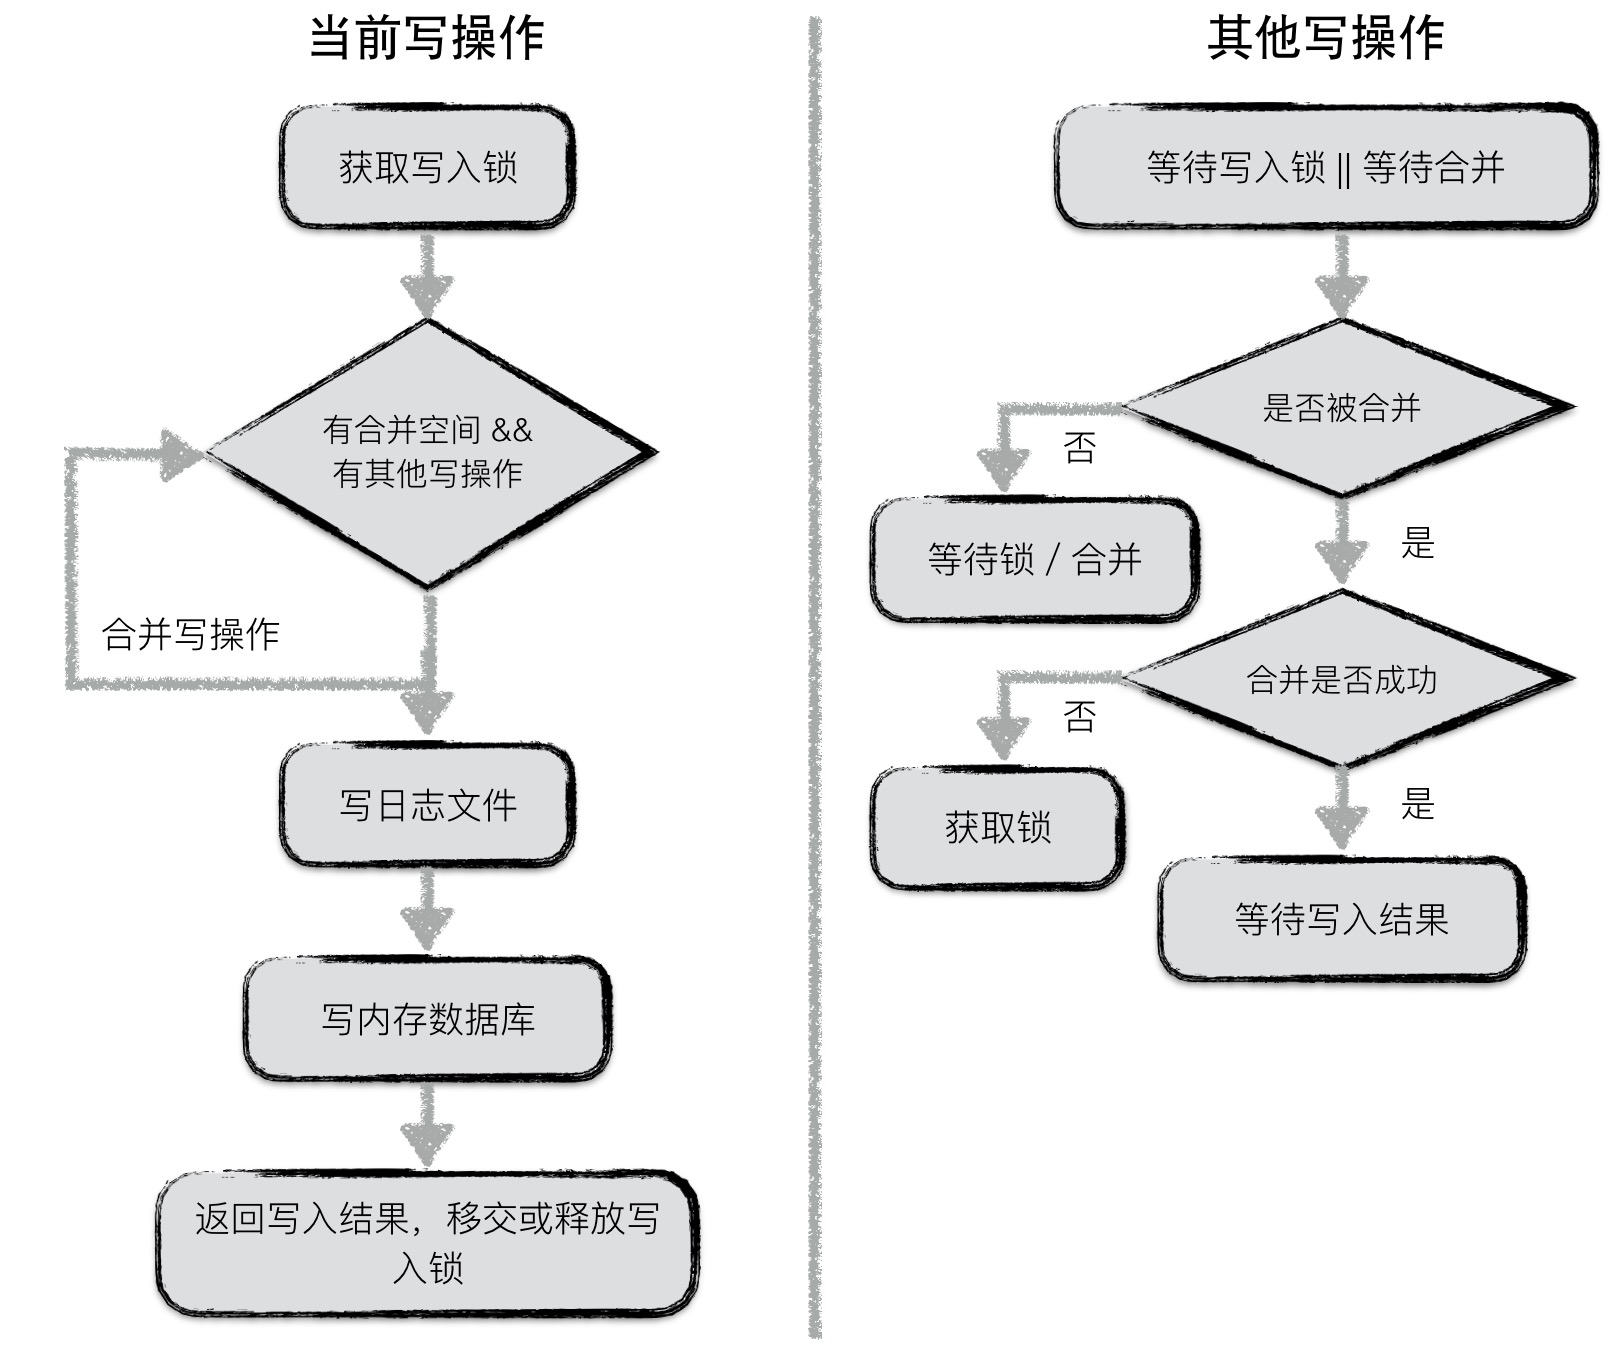
\includegraphics[width=0.95\textwidth]{images/write_merge}
			\caption{写合并的流程}
			\label{write_merge}
		\end{figure}

		\item 原子性
		
		存储系统的任意一个写操作(无论包含了多少次写),其原子性都是由日志文件实现的。
		一个写操作中所有的内容会以一个日志中的一条记录,作为最小单位写入。

		考虑以下两种异常情况:

		(1)写日志未开始,或写日志完成一半,进程异常退出;
		(2)写日志完成,进程异常退出;

		前者中可能存储一个写操作的部分写已经被记载到日志文件中,仍然有部分写未被记录,
		这种情况下,当数据库重新启动恢复时,读到这条日志记录时,发现数据异常,直接丢弃或退出,
		实现了写入的原子性保障。

		后者,写日志已经完成,写入日志的数据未真正持久化,
		存储系统启动恢复时通过redo日志实现数据写入,仍然保障了原子性。

		\end{enumerate}


		\subsubsection{读数据的实现}

	存储系统提供给用户两种进行读取数据的接口:

	直接通过Get接口读取数据;
	首先创建一个snapshot,基于该snapshot调用Get接口读取数据;
	两者的本质是一样的,只不过第一种调用方式默认地以当前数据库的状态创建了一个snapshot,
	并基于此snapshot进行读取。

	读者可能不了解snapshot(快照)到底是什么?简单地来说,就是数据库在某一个时刻的状态。
	基于一个快照进行数据的读取,读到的内容不会因为后续数据的更改而改变。
	
	由于两种方式本质都是基于快照进行读取的,因此在介绍读操作之前,首先介绍快照。

		\begin{enumerate}
		\item snapshot(快照)
		
		快照代表着数据库某一个时刻的状态,在存储系统中,巧妙地用一个整型数来代表一个数据库状态。

		在存储系统中,用户对同一个key的若干次修改(包括删除)是以维护多条数据项的方式进行存储的(直至进行compaction时才会合并成同一条记录),
		每条数据项都会被赋予一个序列号,代表这条数据项的新旧状态。一条数据项的序列号越大,
		表示其中代表的内容为最新值。

		因此,每一个序列号,其实就代表着存储系统的一个状态。
		换句话说,每一个序列号都可以作为一个状态快照。

		当用户主动或者被动地创建一个快照时,存储系统会以当前最新的序列号对其赋值。
		例如图中用户在序列号为98的时刻创建了一个快照,
		并且基于该快照读取key为“name”的数据时,即便此刻用户将"name"的值修改为"dog",
		再删除,用户读取到的内容仍然是“cat”。

		\begin{figure}[H]
			\centering
			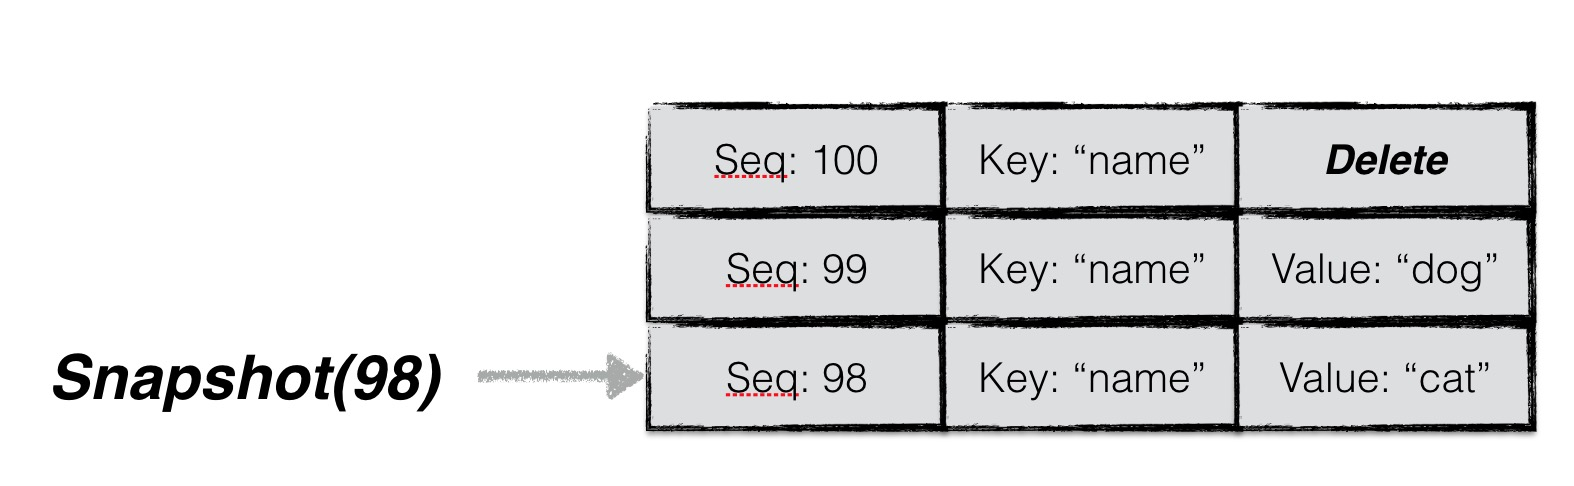
\includegraphics[width=0.95\textwidth]{images/snapshot}
			\caption{快照数据示例图}
			\label{snapshot}
		\end{figure}

		所以,利用快照能够保证数据库进行并发的读写操作。

		在获取到一个快照之后,存储系统会为本次查询的key构建一个internalKey(格式如上文所述),
		其中internalKey的seq字段使用的便是快照对应的seq。
		通过这种方式可以过滤掉所有seq大于快照号的数据项。
		

		\item 读数据流程
		
		\begin{figure}[H]
			\centering
			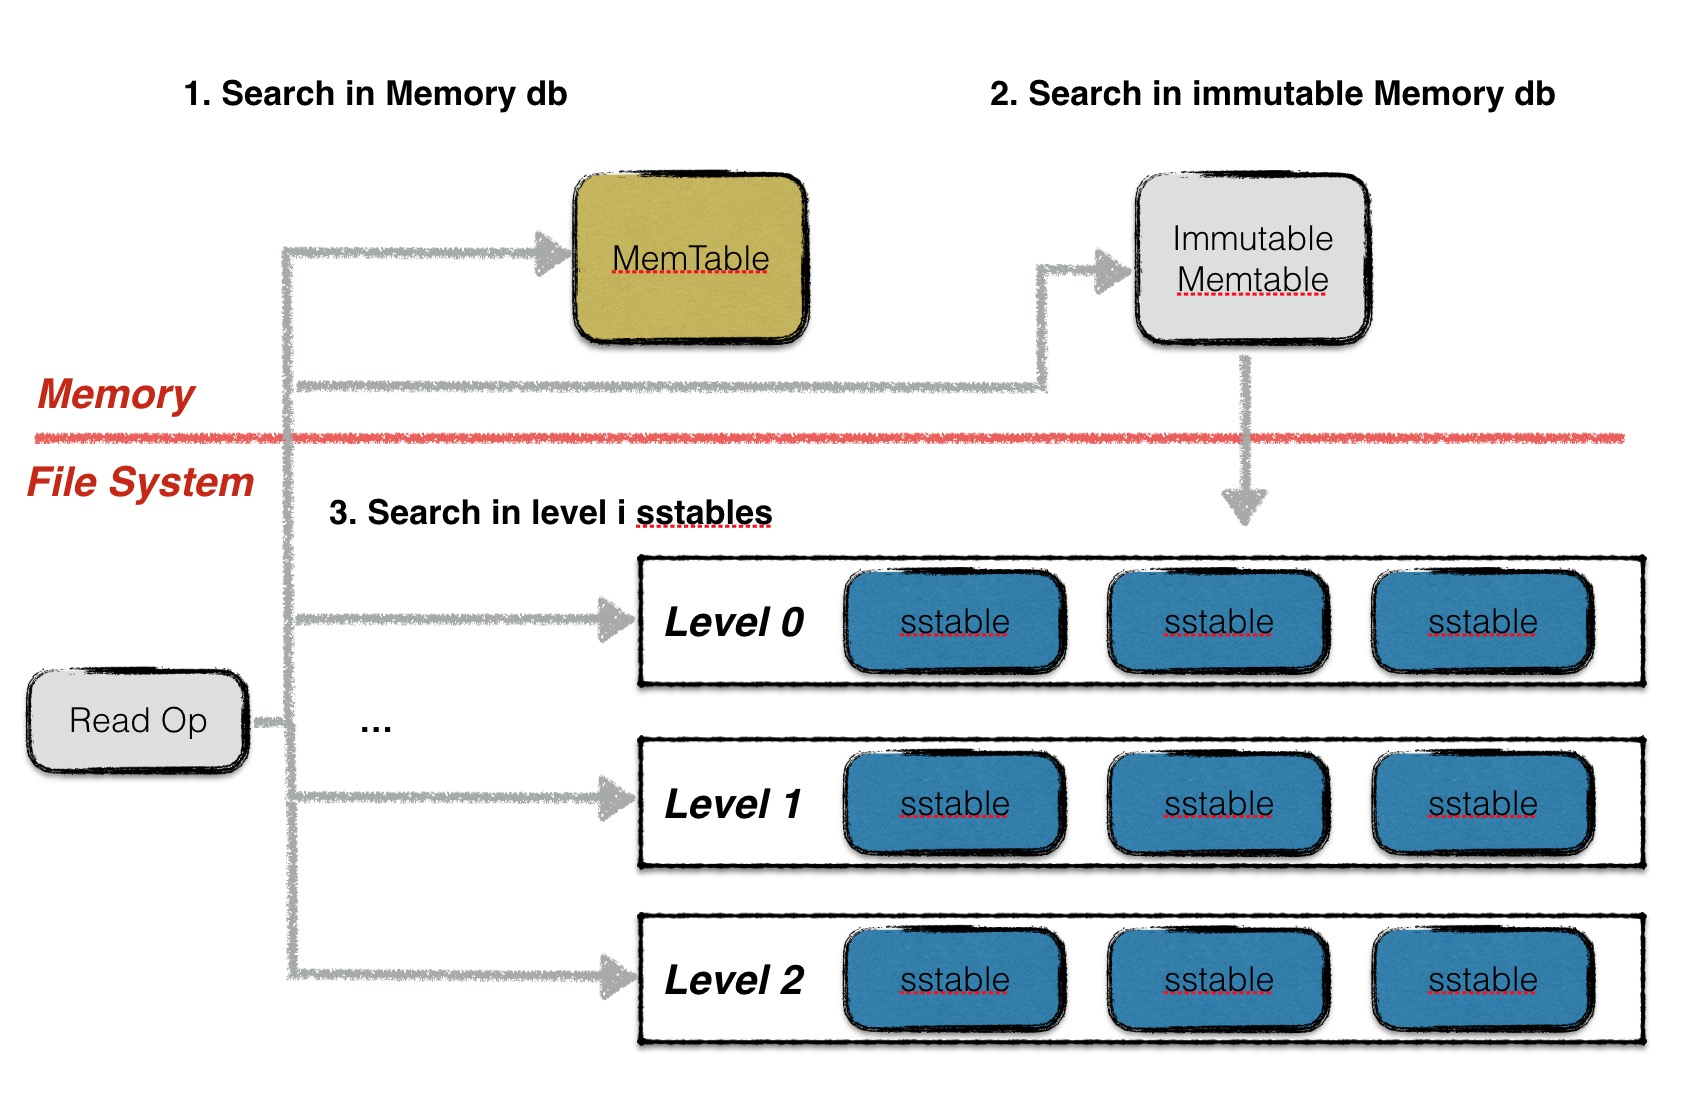
\includegraphics[width=0.95\textwidth]{images/readop}
			\caption{读数据流程}
			\label{readop}
		\end{figure}

		存储系统读取分为三步:

		(1)在memory db中查找指定的key,若搜索到符合条件的数据项,结束查找;

		(2)在冻结的memory db中查找指定的key,若搜索到符合条件的数据项,结束查找;
		
		(3)按低层至高层的顺序在level i层的sstable文件中查找指定的key,
		若搜索到符合条件的数据项,结束查找,否则返回Not Found错误,表示数据库中不存在指定的数据;

		注意存储系统在每一层sstable中查找数据时,都是按序依次查找sstable的。

		0层的文件比较特殊。由于0层的文件中可能存在key重合的情况,
		因此在0层中,文件编号大的sstable优先查找。
		理由是文件编号较大的sstable中存储的总是最新的数据。

		非0层文件,一层中所有文件之间的key不重合,
		因此存储系统可以借助sstable的元数据(一个文件中最小与最大的key值)进行快速定位,
		每一层只需要查找一个sstable文件的内容。

		在memory db或者sstable的查找过程中,需要根据指定的序列号拼接一个internalKey,
		查找用户key一致,且seq号不大于指定seq的数据,
		
		\end{enumerate}
	
		\subsubsection{跳表数据结构的实现}

		内存数据库用来维护有序的key-value对,
		其底层是利用跳表实现,绝大多数操作(读/写)的时间复杂度均为O(log n),
		有着与平衡树相媲美的操作效率,但是从实现的角度来说简单许多,
		接下来将介绍一下内存数据库的实现细节。

		\begin{enumerate}
		\item 跳表的实现
		
		跳表(SkipList)是由William Pugh提出的。
		他在论文《Skip lists: a probabilistic alternative to balanced trees》
		中详细地介绍了有关跳表结构、插入删除操作的细节。

		这种数据结构是利用概率均衡技术,加快简化插入、删除操作,
		且保证绝大大多操作均拥有O(log n)的良好效率。
		
		原文的一段话道出了跳表在数据结构中运用离散数学知识的精髓:数据结构是离散的,计算机的本质是离散的。

		\begin{figure}[H]
			\centering
			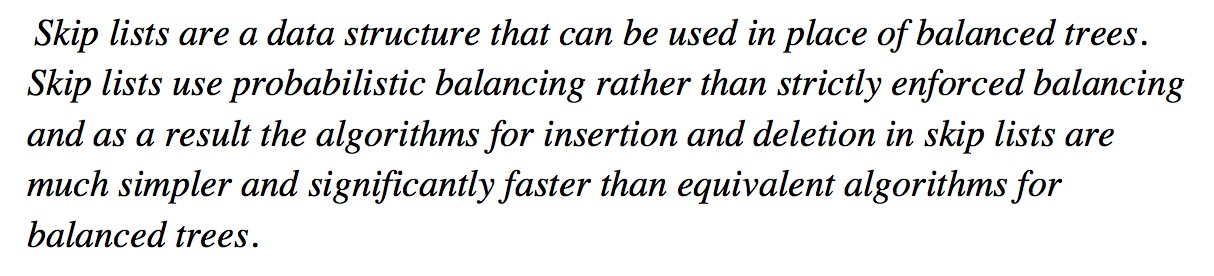
\includegraphics[width=0.95\textwidth]{images/skiplist_effect}
			\caption{跳表的影响}
			\label{skiplist_effect}
		\end{figure}

		平衡树(以红黑树为代表)是一种非常复杂的数据结构,
		为了维持树结构的平衡,获取稳定的查询效率,平衡树每次插入可能会涉及到较为复杂的节点旋转等操作。
		作者设计跳表的目的就是借助概率平衡,来构建一个快速且简单的数据结构,取代平衡树。

		\begin{figure}[H]
			\centering
			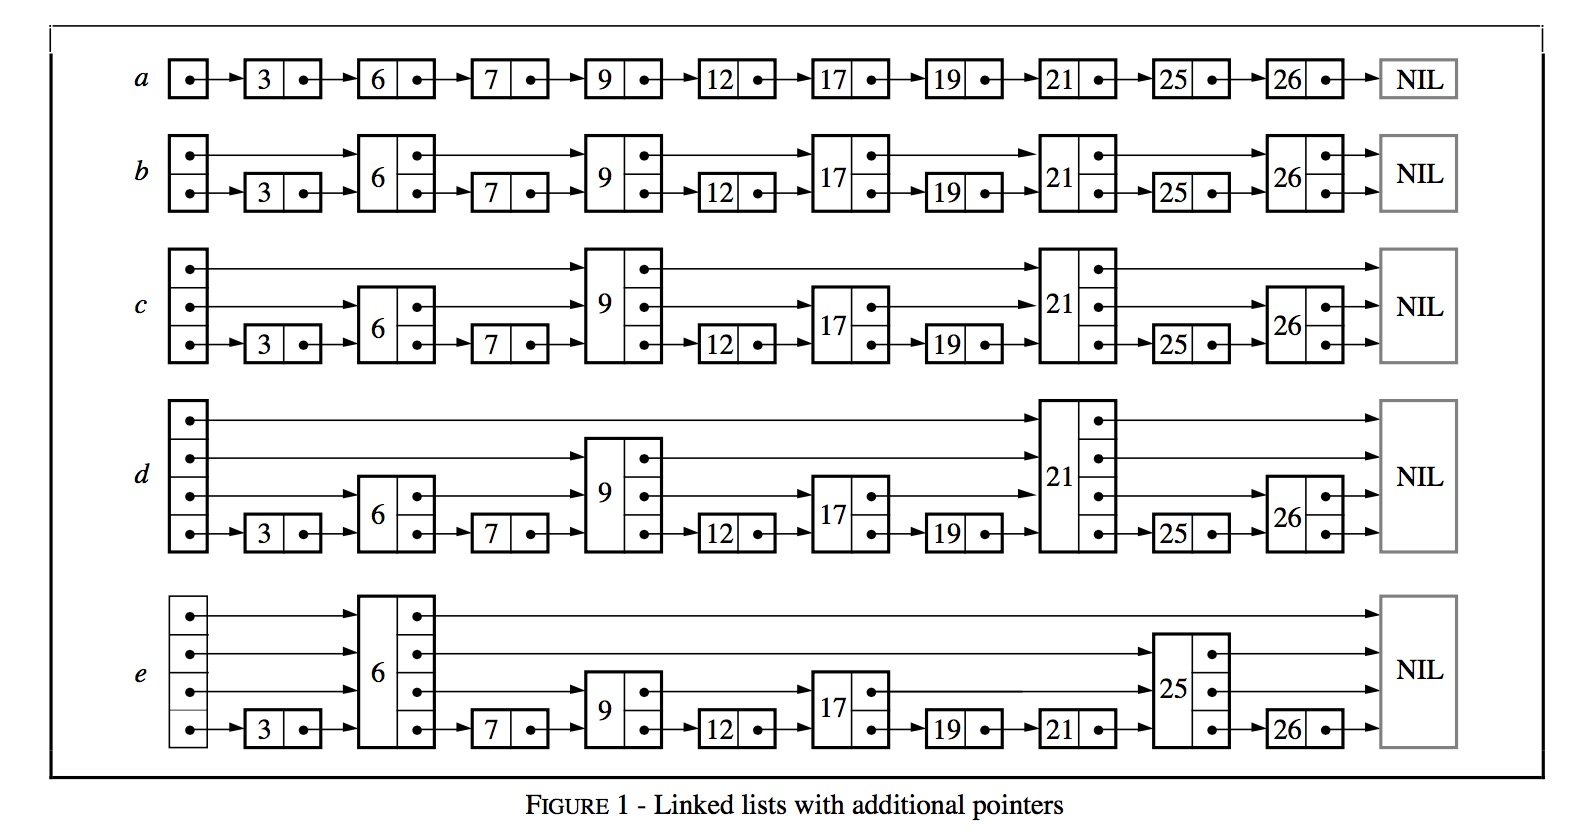
\includegraphics[width=0.95\textwidth]{images/skiplist_intro}
			\caption{一个跳表的图}
			\label{skiplist_intro}
		\end{figure}

		作者从链表讲起,一步步引出了跳表这种结构的由来。

		图a中,所有元素按序排列,被存储在一个链表中,则一次查询之多需要比较N个链表节点;

		图b中,每隔2个链表节点,新增一个额外的指针,该指针指向间距为2的下一个节点,如此以来,借助这些额外的指针,一次查询至多只需要⌈n/2⌉ + 1次比较;

		图c中,在图b的基础上,每隔4个链表节点,新增一个额外的指针,指向间距为4的下一个节点,一次查询至多需要⌈n/4⌉ + 2次比较;

		作者推论,若每隔2个节点,新增一个辅助指针,最终一次节点的查询效率为O(log n)。但是这样不断地新增指针,使得一次插入、删除操作将会变得非常复杂。

		一个拥有k个指针的结点称为一个k层结点(level k node)。按照上面的逻辑,50\% 的结点为1层节点,25\% 的结点为2层节点,12.5\%。
		若保证每层节点的分布如上述概率所示,则仍然能够相同的查询效率。图e便是一个示例。

		维护这些辅助指针将会带来较大的复杂度,因此作者将每一层中,
		每个节点的辅助指针指向该层中下一个节点。
		故在插入删除操作时,只需跟操作链表一样,修改相关的前后两个节点的内容即可完成,
		作者将这种数据结构称为跳表。


		\item 跳表的结构
		
		\begin{figure}[H]
			\centering
			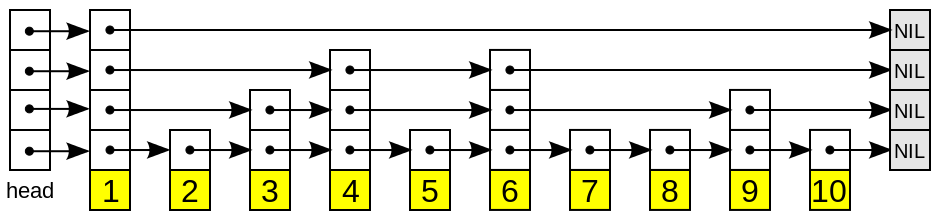
\includegraphics[width=0.95\textwidth]{images/skiplist_arch}
			\caption{跳表的结构}
			\label{skiplist_arch}
		\end{figure}

		跳跃列表是按层建造的。
		底层是一个普通的有序链表。
		每个更高层都充当下面链表的"快速通道",
		这里在层 i 中的元素按某个固定的概率 p (通常为0.5或0.25)出现在层 i+1 中。
		平均起来,每个元素都在 1/(1-p) 个列表中出现,
		而最高层的元素(通常是在跳跃列表前端的一个特殊的头元素)在 O(log1/p n) 个列表中出现。

		\item 跳表的查找
		
		\begin{figure}[H]
			\centering
			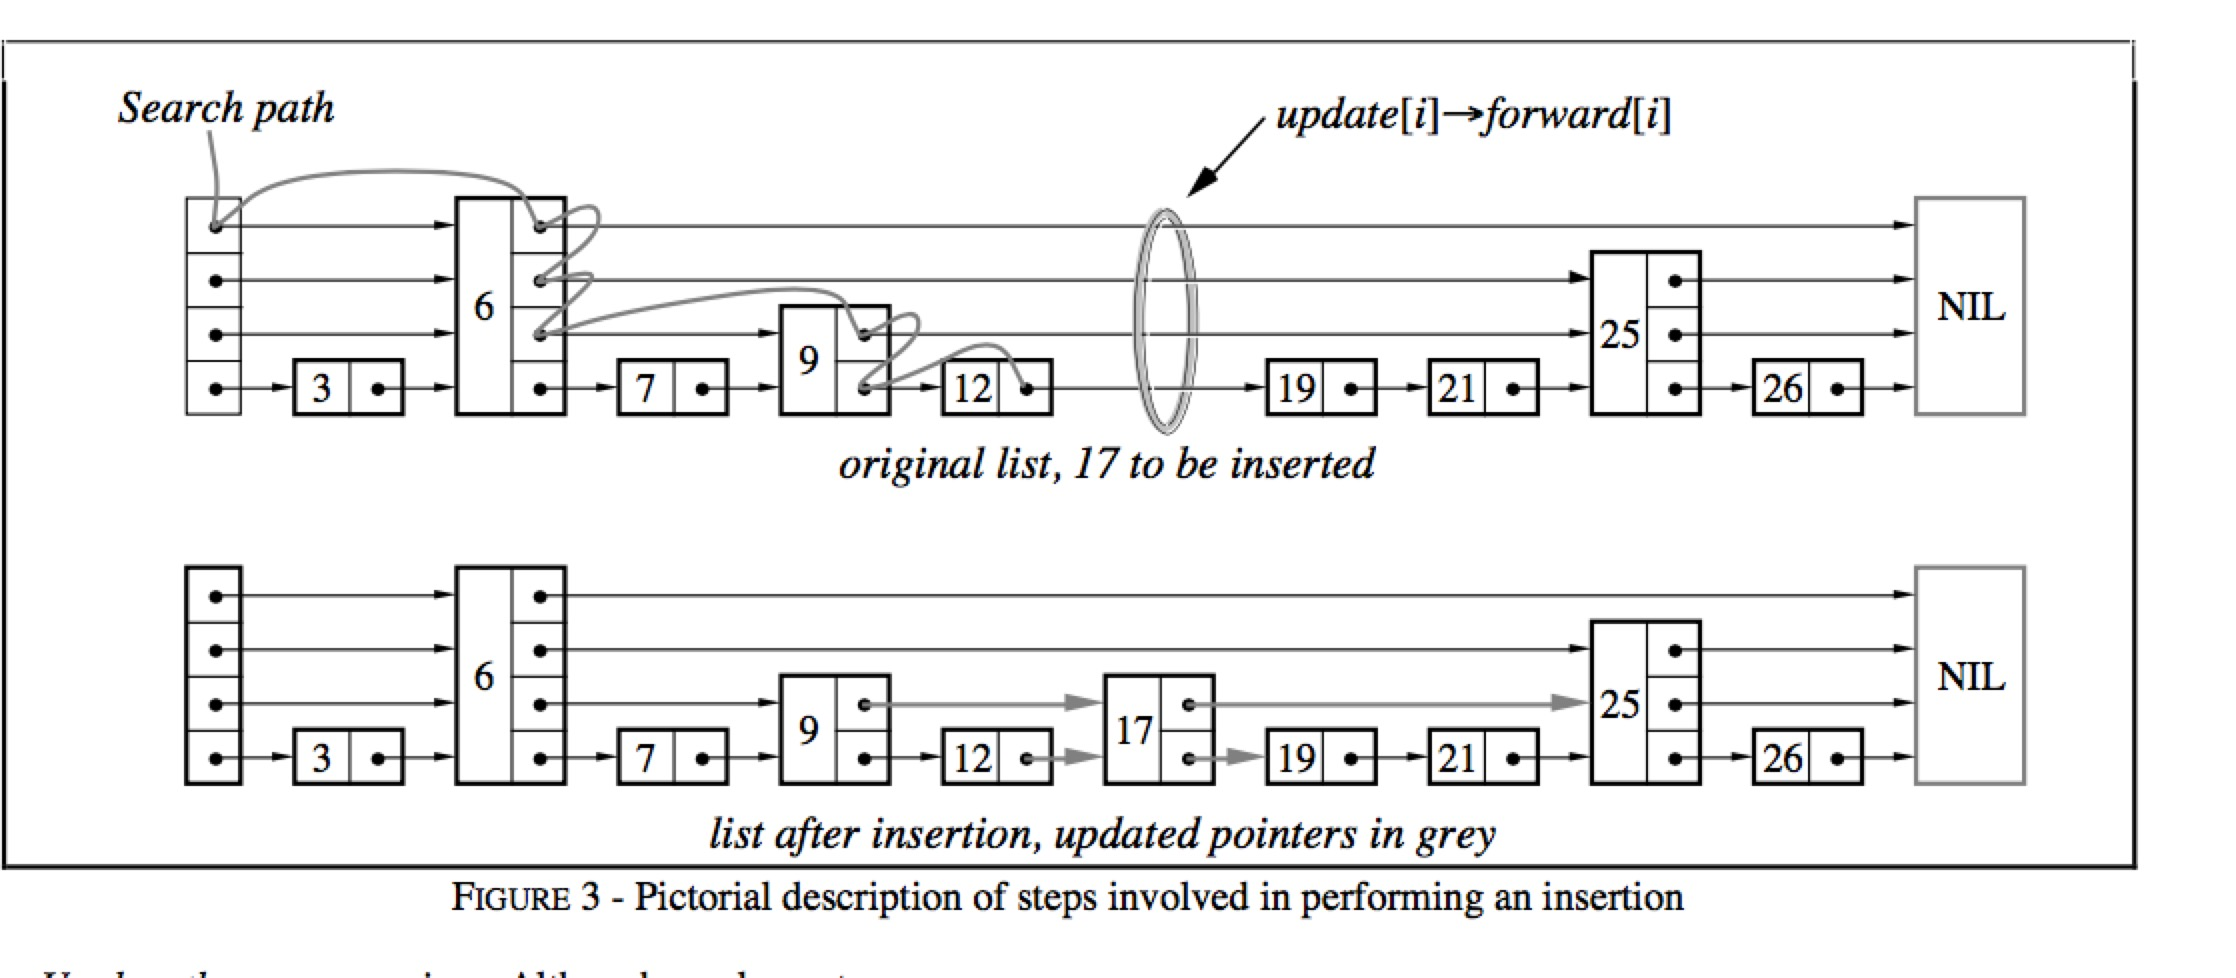
\includegraphics[width=0.95\textwidth]{images/skiplist_search}
			\caption{跳表的查找图}
			\label{skiplist_search}
		\end{figure}
		
		在介绍插入和删除操作之前,我们首先介绍查找操作,该操作是上述两个操作的基础。

例如图中,需要查找一个值为17的链表节点,查找的过程为:

首先根据跳表的高度选取最高层的头节点;

若跳表中的节点内容小于查找节点的内容,则取该层的下一个节点继续比较;

若跳表中的节点内容等于查找节点的内容,则直接返回;

若跳表中的节点内容大于查找节点的内容,且层高不为0,则降低层高,
且从前一个节点开始,重新查找低一层中的节点信息;若层高为0,则返回当前节点,
该节点的key大于所查找节点的key。

综合来说,就是利用稀疏的高层节点,快速定位到所需要查找节点的大致位置,
再利用密集的底层节点,具体比较节点的内容。
		

		\item 跳表的插入
		
		跳表的插入以查找为基础实现

		\begin{figure}[H]
			\centering
			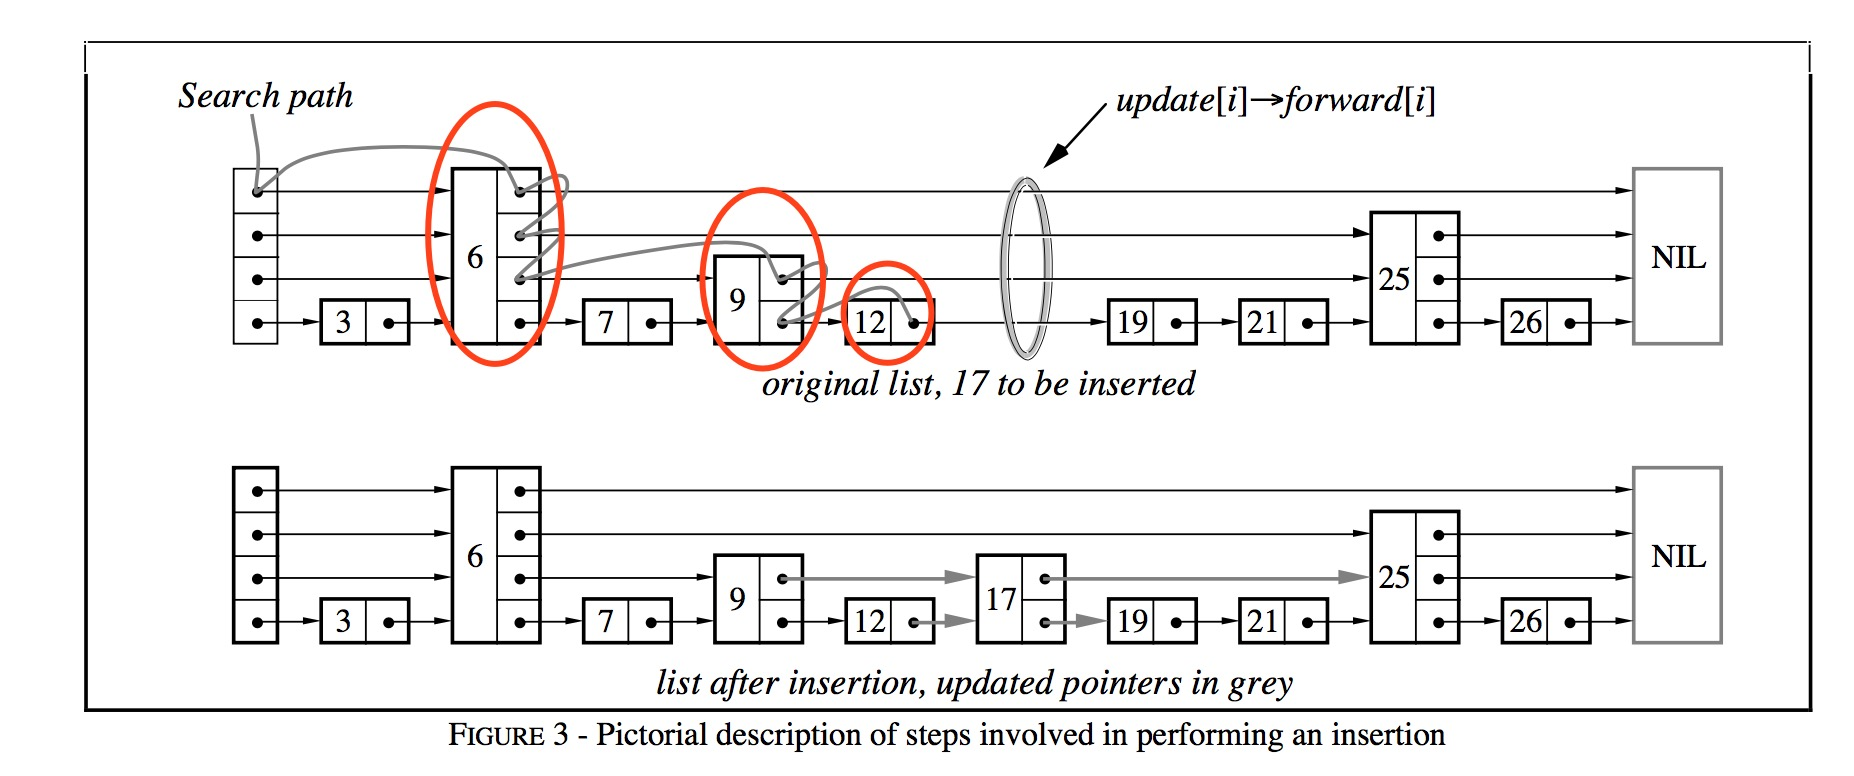
\includegraphics[width=0.95\textwidth]{images/skiplist_insert}
			\caption{跳表的插入图}
			\label{skiplist_insert}
		\end{figure}

		在查找的过程中,不断记录每一层的前任节点,如图中红色圆圈所表示的;
		为新插入的节点随机产生层高(随机产生层高的算法较为简单,依赖最高层数和概率值p,可见下文中的代码实现);
		在合适的位置插入新节点(例如图中节点12与节点19之间),并依据查找时记录的前任节点信息,
		在每一层中,以链表插入的方式,将该节点插入到每一层的链接中。


		链表插入指:将当前节点的Next值置为前任节点的Next值,将前任节点的Next值替换为当前节点。

		\begin{lstlisting}[caption=skiplistRandHeight , label=code_radds_storage_skiplist_randHeight]
func (p *DB) randHeight() (h int) {
	const branching = 4
	h = 1
	for h < tMaxHeight && p.rnd.Int()%branching == 0 {
		h++
	}
	return
}	
		\end{lstlisting}

		\item 跳表的删除

		跳表的删除操作较为简单,依赖查找过程找到该节点在整个跳表中的位置后,以链表删除的方式,
		在每一层中,删除该节点的信息。

		链表删除指:将前任节点的Next值替换为当前节点的Next值,并将当前节点所占的资源释放。

		\item 跳表的迭代
		
		(1)向后遍历

		若迭代器刚被创建,则根据用户指定的查找范围[Start, Limit)找到一个符合条件的跳表节点;
		
		若迭代器处于中部,则取出上一次访问的跳表节点的后继节点,
		作为本次访问的跳表节点(后继节点为最底层的后继节点);
		
		利用跳表节点信息(keyvalue数据偏移量,key,value值长度等),获取keyvalue数据;
		
		(2)向前遍历

		若迭代器刚被创建,则根据用户指定的查找范围[Start, Limit)在跳表中找到最后一个符合条件的跳表节点;
		
		若迭代器处于中部,则利用上一次访问的节点的key值,查找比该key值更小的跳表节点;
		
		利用跳表节点信息(keyvalue数据偏移量,key,value值长度等),获取keyvalue数据;

	\end{enumerate}

		\subsubsection{内存数据库的实现}

		在介绍完跳表这种数据结构的组织原理以后,我们介绍存储系统如何利用跳表来构建一个高效的内存数据库。

		\begin{enumerate}
			\item 键值编码
			
			在介绍内存数据库之前,首先介绍一下内存数据库的键值编码规则。
			由于内存数据库本质是一个kv集合,且所有的数据项都是依据key值排序的,因此键值的编码规则尤为关键。

			内存数据库中,key称为internalKey,其由三部分组成:

			用户定义的key:这个key值也就是原生的key值;
			
			序列号:存储系统中,每一次写操作都有一个sequence number,标志着写入操作的先后顺序。
			由于在存储系统中可能会有多条相同key的数据项同时存储在数据库中,
			因此需要有一个序列号来标识这些数据项的新旧情况。序列号最大的数据项为最新值;
			
			类型:标志本条数据项的类型,为更新还是删除;

			\begin{figure}[H]
				\centering
				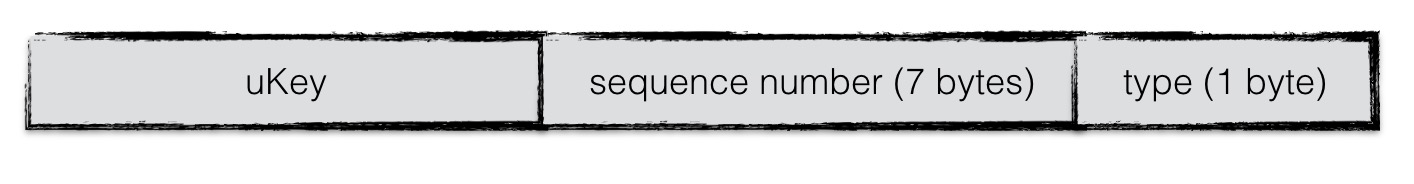
\includegraphics[width=0.95\textwidth]{images/internalkey}
				\caption{内存数据库内部键}
				\label{internalkey}
			\end{figure}

			\item 键值比较
			
			内存数据库中所有的数据项都是按照键值比较规则进行排序的。
			这个比较规则可以由用户自己定制,也可以使用系统默认的。在这里介绍一下系统默认的比较规则。

			默认的比较规则:

			首先按照字典序比较用户定义的key(ukey),若用户定义key值大,整个internalKey就大;
			
			若用户定义的key相同,则序列号大的internalKey值就小;
			
			通过这样的比较规则,则所有的数据项首先按照用户key进行升序排列;
			当用户key一致时,按照序列号进行降序排列,这样可以保证首先读到序列号大的数据项。


			\item 数据组织
			
			\begin{lstlisting}{caption=storage_db, label=code_radds_storage_db}
type DB struct {
	cmp comparer.BasicComparer
	rnd *rand.Rand
	mu     sync.RWMutex
	kvData []byte
	// Node data:
	// [0]         : KV offset
	// [1]         : Key length
	// [2]         : Value length
	// [3]         : Height
	// [3..height] : Next nodes
	nodeData  []int
	prevNode  [tMaxHeight]int
	maxHeight int
	n         int
	kvSize    int
}
		\end{lstlisting}
				
			
			其中kvData用来存储每一条数据项的key-value数据,nodeData用来存储每个跳表节点的链接信息。

			nodeData中,每个跳表节点占用一段连续的存储空间,每一个字节分别用来存储特定的跳表节点信息。

			第一个字节用来存储本节点key-value数据在kvData中对应的偏移量;
			
			第二个字节用来存储本节点key值长度;
			
			第三个字节用来存储本节点value值长度;
			
			第四个字节用来存储本节点的层高;
			
			第五个字节开始,用来存储每一层对应的下一个节点的索引值;

		\item 基础操作
		
		Put、Get、Delete、Iterator等操作均依赖于底层的跳表的基本操作实现,不再赘述。
		\end{enumerate}

		\subsubsection{持久化数据存储的实现}

			\begin{enumerate}
				\item sstable概述
				
				如我们之前提到的,系统是的LSM树(Log Structured-Merge Tree)实现,
				即一次写入过程并不是直接将数据持久化到磁盘文件中,而是将写操作首先写入日志文件中,
				其次将写操作应用在memtable上。

				当其达到checkpoint点(memtable中的数据量超过了预设的阈值),
				会将当前memtable冻结成一个不可更改的内存数据库
				(immutable memory db),并且创建一个新的memtable供系统继续使用。

				immutable memory db会在后台进行一次minor compaction,
				即将内存数据库中的数据持久化到磁盘文件中。

				LSM树设计Minor Compaction的目的是为了:

				有效地降低内存的使用率;
				
				避免日志文件过大,系统恢复时间过长;
				
				当memory db的数据被持久化到文件中时,
				leveldb将以一定规则进行文件组织,这种文件格式成为sstable。
				在本文中将详细地介绍sstable的文件格式以及相关读写操作。

				\item sstable文件格式
				
				物理结构

				为了提高整体的读写效率,一个sstable文件按照固定大小进行块划分,默认每个块的大小为4KiB。
				每个Block中,除了存储数据以外,还会存储两个额外的辅助字段:

				(1)压缩类型

				(2)CRC校验码

				压缩类型说明了Block中存储的数据是否进行了数据压缩,
				若是,采用了哪种算法进行压缩。leveldb中默认采用Snappy算法进行压缩。

				CRC校验码是循环冗余校验校验码,校验范围包括数据以及压缩类型。
				
				\begin{figure}[H]
					\centering
					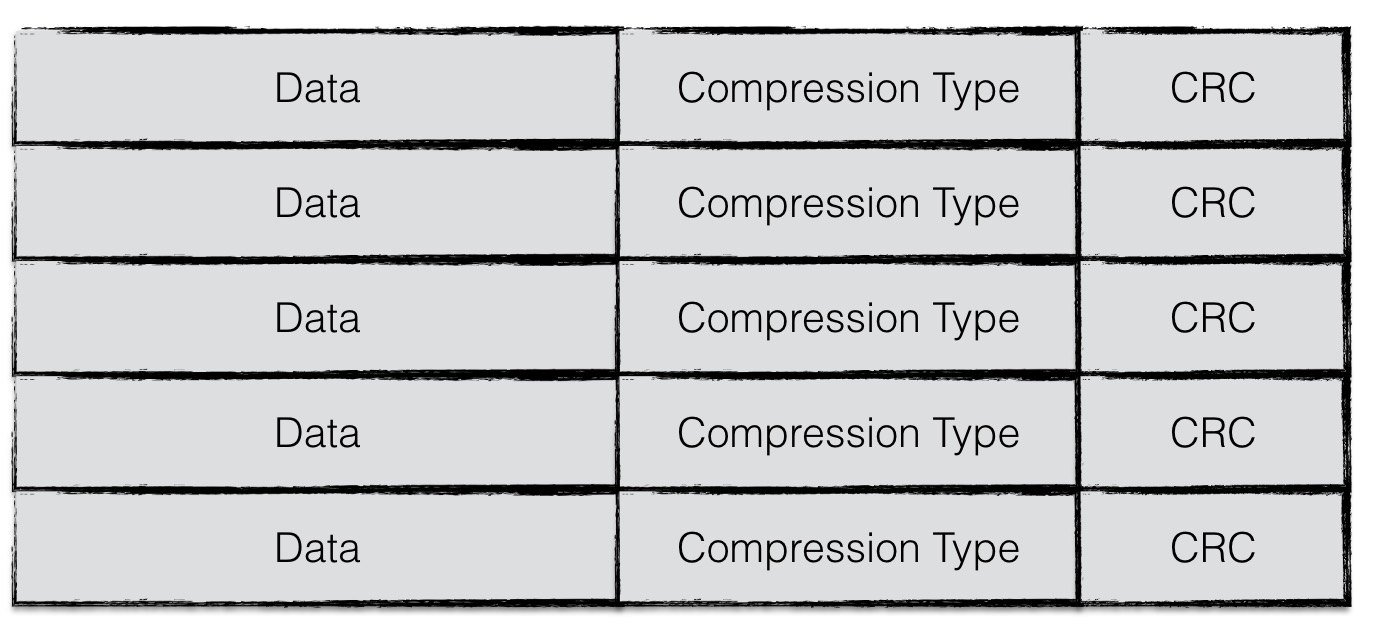
\includegraphics[width=0.95\textwidth]{images/sstable_physic.jpeg}
					\caption{sstable物理结构}
					\label{sstable_physic}
				\end{figure}
				
				逻辑结构

				在逻辑上,根据功能不同,leveldb在逻辑上又将sstable分为:

data block: 用来存储key value数据对;

filter block: 用来存储一些过滤器相关的数据(布隆过滤器),但是若用户不指定leveldb使用过滤器,leveldb在该block中不会存储任何内容;

meta Index block: 用来存储filter block的索引信息(索引信息指在该sstable文件中的偏移量以及数据长度);

index block:index block中用来存储每个data block的索引信息;

footer: 用来存储meta index block及index block的索引信息;

\begin{figure}[H]
	\centering
	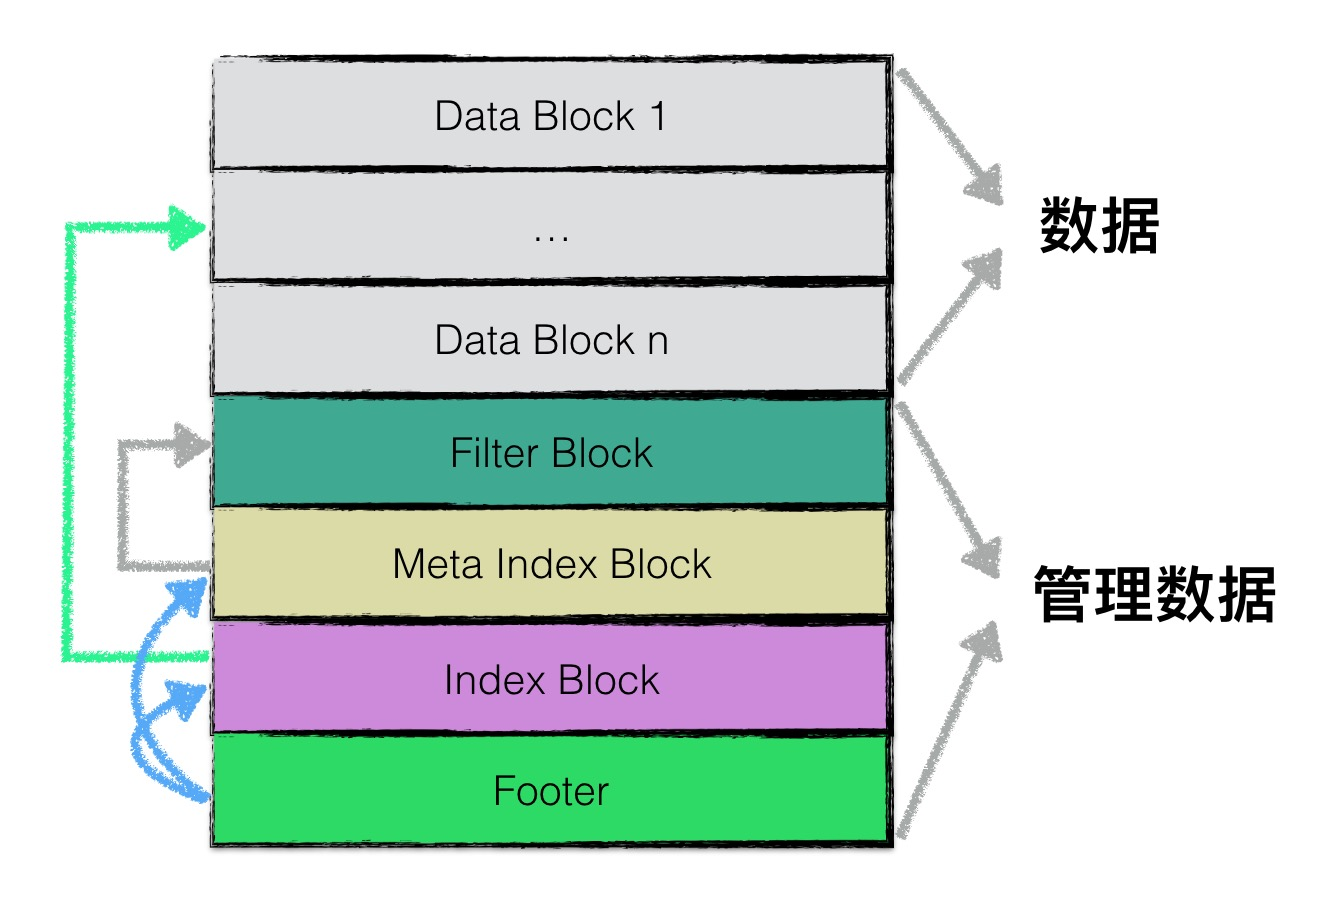
\includegraphics[width=0.95\textwidth]{images/sstable_logic.jpeg}
	\caption{sstable逻辑结构}
	\label{sstable_logic}
\end{figure}

			每个区块都会有自己的压缩信息以及CRC校验码信息。

				datablock结构

				data block中存储的数据是leveldb中的keyvalue键值对。
				其中一个data block中的数据部分(不包括压缩类型、CRC校验码)按逻辑又以下图进行划分:
				
				\begin{figure}[H]
					\centering
					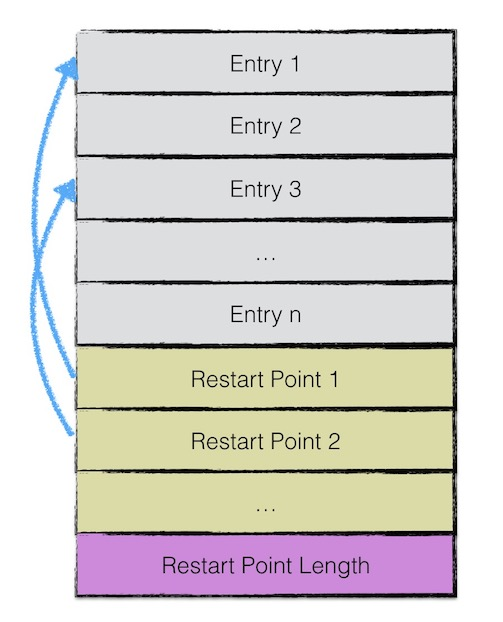
\includegraphics[width=0.95\textwidth]{images/datablock.jpeg}
					\caption{sstable data block}
					\label{sstable_data_block}
				\end{figure}
				
				第一部分用来存储keyvalue数据。由于sstable中所有的keyvalue对都是严格按序存储的,
				为了节省存储空间,leveldb并不会为每一对keyvalue对都存储完整的key值,而是存储与上一个key非共享的部分,
				避免了key重复内容的存储。

				每间隔若干个keyvalue对,将为该条记录重新存储一个完整的key。
				重复该过程(默认间隔值为16),
				每个重新存储完整key的点称之为Restart point。

				leveldb设计Restart point的目的是在读取sstable内容时,
				加速查找的过程。

				由于每个Restart point存储的都是完整的key值,
				因此在sstable中进行数据查找时,
				可以首先利用restart point点的数据进行键值比较,
				以便于快速定位目标数据所在的区域;

				当确定目标数据所在区域时,
				再依次对区间内所有数据项逐项比较key值,进行细粒度地查找;
				该思想有点类似于跳表中利用高层数据迅速定位,
				底层数据详细查找的理念,降低查找的复杂度。

				
				每个数据项格式如下图所示:

				\begin{figure}[H]
					\centering
					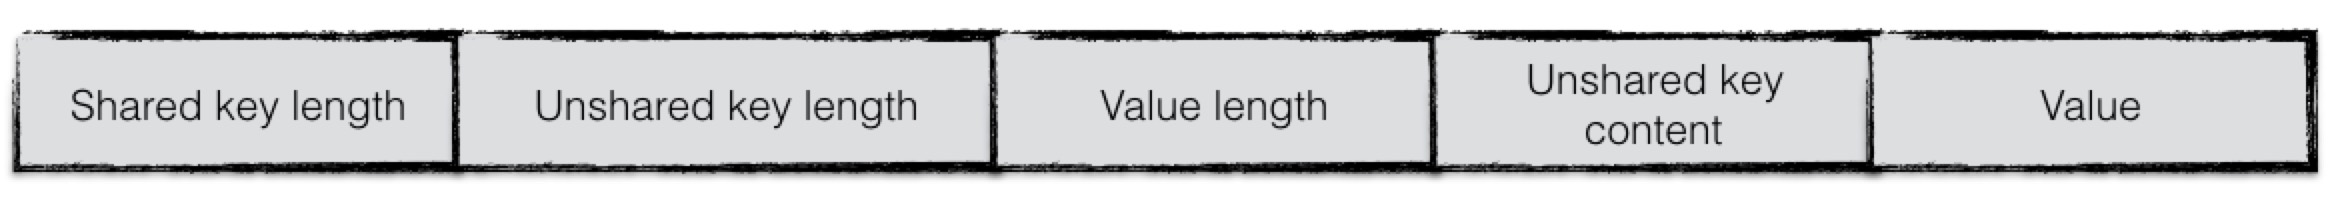
\includegraphics[width=0.95\textwidth]{images/entry_format.jpeg}
					\caption{sstable entry format}
					\label{sstable_entry_format}
				\end{figure}

				一个entry分为5部分内容:

与前一条记录key共享部分的长度;

与前一条记录key不共享部分的长度;

value长度;

与前一条记录key非共享的内容;

value内容;

\begin{figure}[H]
	\centering
	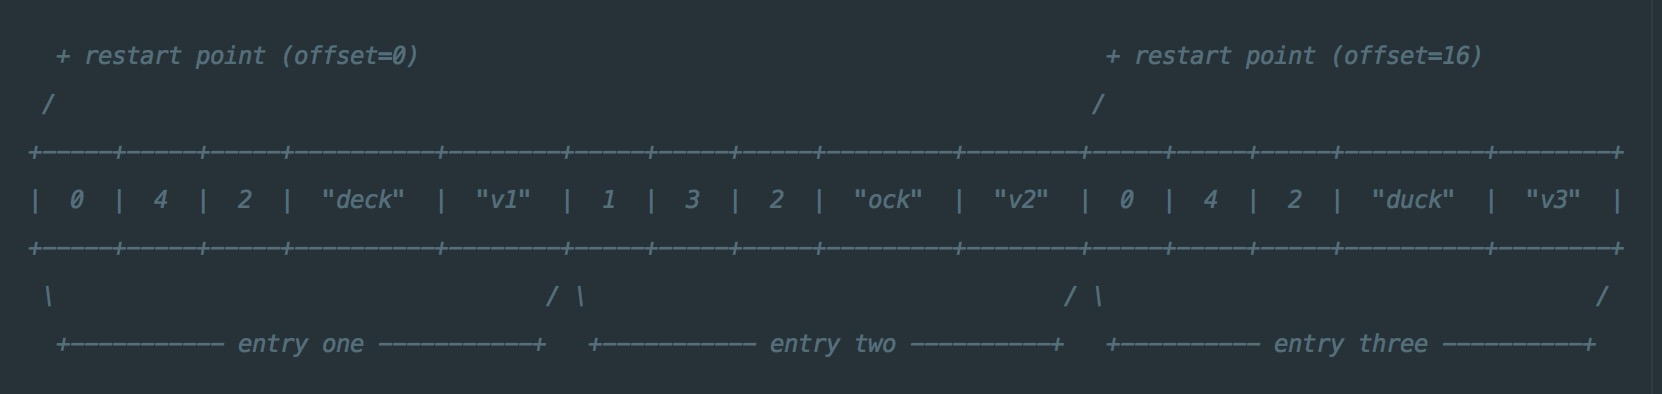
\includegraphics[width=0.95\textwidth]{images/datablock_example_1.jpeg}
	\caption{sstable data block 示例图1}
	\label{sstable_datablock_example_1}
\end{figure}


三组entry按上图的格式进行存储。
值得注意的是restart\_interval为2,
因此每隔两个entry都会有一条数据作为restart point点的数据项,
存储完整key值。因此entry3存储了完整的key。

此外,第一个restart point为0(偏移量),第二个restart point为16,
restart point共有两个,
因此一个datablock数据段的末尾添加了下图所示的数据:

\begin{figure}[H]
	\centering
	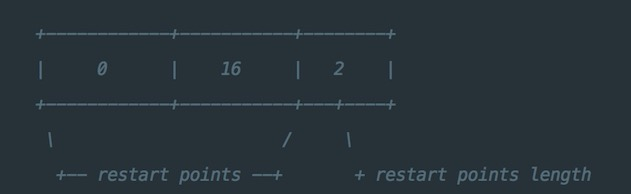
\includegraphics[width=0.95\textwidth]{images/datablock_example_2.jpeg}
	\caption{sstable data block 示例图2}
	\label{sstable_datablock_example_2}
\end{figure}

尾部数据记录了每一个restart point的值,以及所有restart point的个数。

filter block结构

为了加快sstable中数据查询的效率,在直接查询datablock中的内容之前,
leveldb首先根据filter block中的过滤数据判断指定的datablock中是否有需要查询的数据,
若判断不存在,则无需对这个datablock进行数据查找。

filter block存储的是data block数据的一些过滤信息。
这些过滤数据一般指代布隆过滤器的数据,用于加快查询的速度,

filter block存储的数据主要可以分为两部分:(1)过滤数据(2)索引数据。

其中索引数据中,filter i offset表示第i个filter data在整个filter block中的起始偏移量,filter offset's offset表示filter block的索引数据在filter block中的偏移量。

在读取filter block中的内容时,可以首先读出filter offset's offset的值,然后依次读取filter i offset,根据这些offset分别读出filter data。

Base Lg默认值为11,表示每2KB的数据,创建一个新的过滤器来存放过滤数据。

一个sstable只有一个filter block,其内存储了所有block的filter数据。
具体来说,filter\_data\_k 包含了所有起始位置处于 [base*k, base*(k+1)]
范围内的block的key的集合的filter数据,
按数据大小而非block切分主要是为了尽量均匀,
以应对存在一些block的key很多,另一些block的key很少的情况。


				\item sstable读写操作
				


				\item sstable文件特点
			\end{enumerate}


		\subsubsection{缓存系统的实现}


		\subsubsection{布隆过滤器的实现}

		\subsubsection{数据压缩系统的实现}

		\subsubsection{版本控制的实现}

	